\documentclass[10pt]{article}

\usepackage[utf8]{inputenc}
\usepackage[T1]{fontenc}
\usepackage[english]{babel} % If needed, change language here
\usepackage{amssymb}
\usepackage{color}
\usepackage{graphicx}
\usepackage{caption}
\usepackage[obeyFinal]{easy-todo}
\usepackage{subcaption}
\usepackage{url}
\usepackage{nameref}
\usepackage[bottom, symbol]{footmisc} % footnotes to the bottom of the page
\usepackage{tablefootnote}
\renewcommand{\thefootnote}{\fnsymbol{footnote}}

% Optional: decrease margins to fit more on one page
\usepackage{geometry}
\geometry{
	a4paper,
	total={190mm,257mm},
%	left=15mm,
%	top=15mm,
%	right=15mm,
%	bottom=15mm
}

% Place todo's using \todo
%\newcommand{\todo}{{\color{red}{\textbf{TODO }}}}

\newcommand{\plot}[1]{\includegraphics[width=.48\linewidth]{../results/plots/#1}}
\newcommand{\plots}[1]{
	\plot{#1-acc.png} & \plot{#1-exec.png} \\
	\texttt{#1} accuracy & \texttt{#1} execution times \\
}
\newcommand{\sbs}[1]{
	\begin{figure}[ht]
		\begin{subfigure}{.48\linewidth}
			\centering
			\includegraphics[width=\linewidth]{../results/plots/#1-acc-2.png}
			\caption{\texttt{#1} accuracy}
			\label{fig:acc-#1}
		\end{subfigure}%
		\hfill
		\begin{subfigure}{.48\linewidth}
			\centering
			\includegraphics[width=\linewidth]{../results/plots/#1-exec-2.png}
			\caption{\texttt{#1} execution time}
			\label{fig:exec-#1}
		\end{subfigure}
		\caption{Effect of hyperparameters on \texttt{#1} dataset}
		\label{fig:#1}
	\end{figure}
}

\begin{document}
\font\myfont=cmr12 at 15pt

\title{\vspace{-2.5cm}{\myfont Assignment 3: BDAP [B-KUL-H00Y4A]}}
%\author{Andreas Hinderyckx}
\date{} % Choose custom date


\maketitle
%\listoftodos

\vspace{-2cm}
\paragraph{Q1}
The approximate product quantization (PQ) method is faster than the naive nearest neighbors (NN) because it limits the amount of distance computations, which dominate execution time. Concretely: for naive NN $N$ distances are computed per query in the case of $N$ training examples. When using PQNN, the $N$ training instances are mapped onto \texttt{nclusters} centroids $\ll N$. Only the distances between the query example and the \texttt{nclusters} must be calculated (per partition), hence the computation time drops significantly. Thus, although the search is still exhaustive, less memory has to be visited and only $\# partitions$ additions are required per distance calculation, rather than $\# features$ subtractions \textit{and} multiplications\footnote{\url{https://hal.inria.fr/inria-00410767/document/}}.
%Computing distance is summing m numbers vs.
%d subtractions \& multiplications!
%
%memory. Searching the nearest
%neighbors with a product quantizer is faster because less memory has to be visited and only m additions are required per distance calculation, but the search is still exhaustive \url{https://hal.inria.fr/inria-00410767/document/}

\vspace{-.3cm}
\paragraph{Q2} Figure \ref{fig:acc} shows that accuracy increases with the number of partitions and clusters, as these refine the PQ's approximation.
From figure \ref{fig:exec} it can be seen that the execution time grows with the number of clusters and shifts upwards by a constant factor when increasing the number of partitions. 
\vspace{-.4cm}
\begin{figure}[h]
	\begin{subfigure}{.5\textwidth}
		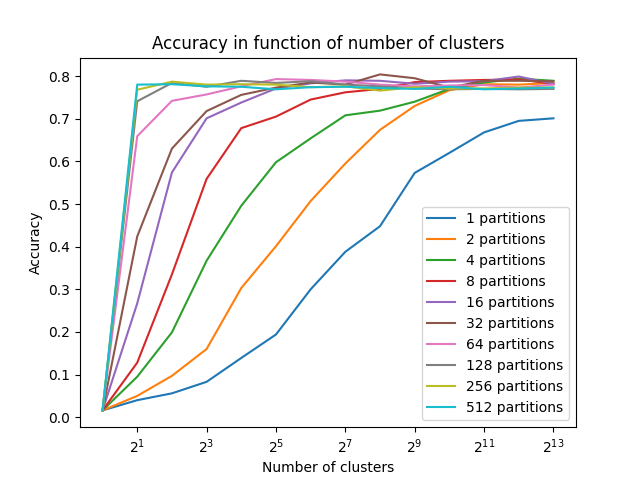
\includegraphics[width=\linewidth]{../results/plots/emnist_orig-acc-2.png}
		\caption{Accuracy on \texttt{emnist\_orig}}
		\label{fig:acc}
	\end{subfigure}%
	\hfill
	\begin{subfigure}{.5\textwidth}
		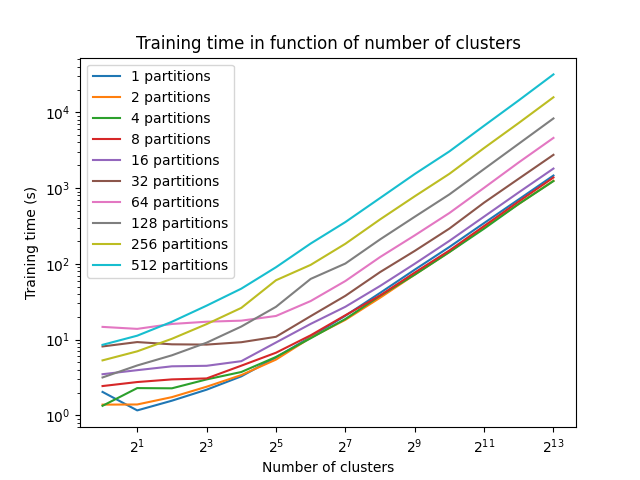
\includegraphics[width=\linewidth]{../results/plots/emnist_orig-exec-2.png}
		\caption{Training time on \texttt{emnist\_orig}}
		\label{fig:exec}
	\end{subfigure}
	\vspace{-.3cm}
	\caption{Effect of number of clusters and number of partitions on accuracy (\ref{fig:acc}) and execution time (\ref{fig:exec}) of \texttt{ProdQuanNN}}
	\label{fig:hyperparams}
\end{figure}

\vspace{-.8cm}
\paragraph{Q3} Purely based on accuracy, \texttt{npartitions} and \texttt{nclusters} should be chosen as large as is needed to achieve the maximum accuracy (cfr. plots \ref{fig:acc} - \ref{fig:acc-higgs}). This increases execution time, however. As such, a trade-off between execution time and accuracy should be made: choosing (\texttt{npartitions}, \texttt{nclusters}) $= (2^4, 2^5)$ for \texttt{emnist\_orig} for example hits $72.5\%$ accuracy ($\sim 96\%$ of its peak accuracy), while still completing in under $10$ seconds. Both hyperparameters should also be chosen sufficiently large to achieve a higher \texttt{retrieval\_rate}.

\vspace{-.35cm}
\paragraph{Q4} The results of the experiments are shown in table \ref{tab:experiments}. The \texttt{seed} and \texttt{k} hyperparameters were left on their default values of \texttt{1} and \texttt{10} respectively, while \texttt{n} was chosen = 1000 to have a representative sample size\footnote{\url{https://stats.stackexchange.com/a/172}}.
\vspace{-.45cm}
\begin{table}[h]
	\centering
	\hspace{-.2cm}\begin{tabular}{l c | c c c c}
		& 
		& \begin{minipage}[t]{.17\linewidth}
			 \centering 
			 \texttt{time\_and\_accuracy}  (\texttt{accuracy}, \texttt{time} [s])
		  \end{minipage}
		& \begin{minipage}[t]{.24\linewidth}
			\centering
			\texttt{distance\_error}\\ (\textit{\textbf{$L^2$}} norm)%\tablefootnote{See code comments for details}
		\end{minipage}
		& \begin{minipage}[t]{.07\linewidth}
			\centering
			\texttt{retrieval} 
		\end{minipage}
		& \begin{minipage}[t]{.3\linewidth}
			\centering
			Optimal hyperparameters (\texttt{npartitions}, \texttt{nclusters}) 
		\end{minipage}\\
		\hline
		\texttt{spambase}     & \texttt{SKLearn} & (0.987, 0.1)  & -        & -   & - \\
						      & \texttt{NumpyNN} & (0.987, 18)   & -        & -   & - \\
						      & \texttt{PQNN}    & (0.986, 4)    & 0.042    & 0.889 & $(2^4, 2^4)$\\\hline
		\texttt{covtype}      & \texttt{SKLearn} & (0.968, 10)   & -        & -   & - \\
						      & \texttt{NumpyNN} & (0.968, 1625) & -        & -   & - \\
						      & \texttt{PQNN}    & (0.952, 194)  & 0.073 & 0.868 & $(2^4, 2^5)$\\\hline
		\texttt{emnist\_orig} & \texttt{SKLearn} & (0.771, 4)    & -        & -   & - \\
							  & \texttt{NumpyNN} & (0.771, 596)  & -        & -   & - \\
						      & \texttt{PQNN}    & (0.783, 177)  & 108.14 & 0.751 & $(2^4, 2^5)$\\\hline
		\texttt{emnist}       & \texttt{SKLearn} & (0.775, 5)    & -        & -   & - \\
						      & \texttt{NumpyNN} & (0.775, 433)  & -        & -   & - \\
						      & \texttt{PQNN}    & (0.784, 130)  & 0.68 & 0.653 & $(2^6,2^6)$\tablefootnote{These hyperparameters can be chosen larger to increase \texttt{retrieval\_rate}, but doing so will supersede \texttt{numpyNN}'s prediction time (due to the large number of features of \texttt{emnist}), nullifying product quantization's performance advantage.}\\\hline
		\texttt{higgs}        & \texttt{SKLearn} & (0.852, 4)    & -        & -   & - \\
							  & \texttt{NumpyNN} & (0.852, 1091) & -        & -   & - \\
						      & \texttt{PQNN}    & (0.859, 428)  & 0.027 & 0.849 & $(2^5,2^5)$\\
	\end{tabular}
	\caption{Experiment results}
	\label{tab:experiments}
\end{table}

%\begin{table}[h]
%	\centering
%	\hspace{-.2cm}\begin{tabular}{l c | c c c c}
%		& 
%		& \begin{minipage}[t]{.17\linewidth}
%			\centering 
%			\texttt{time\_and\_accuracy}  (\texttt{accuracy}, \texttt{time} [s])
%		\end{minipage}
%		& \begin{minipage}[t]{.24\linewidth}
%			\centering
%			\texttt{distance\_error}\\ (\textit{\textbf{$L^2$}} norm, squared \textit{\textbf{$L^2$}} norm)%\tablefootnote{See code comments for details}
%		\end{minipage}
%		& \begin{minipage}[t]{.07\linewidth}
%			\centering
%			\texttt{retrieval} 
%		\end{minipage}
%		& \begin{minipage}[t]{.3\linewidth}
%			\centering
%			Optimal hyperparameters (\texttt{npartitions}, \texttt{nclusters}) 
%		\end{minipage}\\
%		\hline
%		\texttt{spambase}     & \texttt{SKLearn} & (0.987, 0.1)  & -        & -   & - \\
%		& \texttt{NumpyNN} & (0.987, 17)   & -        & -   & - \\
%		& \texttt{PQNN}    & (0.967, 1)    & (0.042, 0.52)    & 0.889 & $(2^3, 2^3)$\\\hline
%		\texttt{covtype}      & \texttt{SKLearn} & (0.968, 10)   & -        & -   & - \\
%		& \texttt{NumpyNN} & (0.968, 1625) & -        & -   & - \\
%		& \texttt{PQNN}    & (0.952, 194)  & (0.073, 0.13) & 0.868 & $(2^4, 2^5)$\\\hline
%		\texttt{emnist\_orig} & \texttt{SKLearn} & (0.771, 4)    & -        & -   & - \\
%		& \texttt{NumpyNN} & (0.771, 596)  & -        & -   & - \\
%		& \texttt{PQNN}    & (0.783, 177)  & (108.14, 2244751.2) & 0.751 & $(2^4, 2^5)$\\\hline
%		\texttt{emnist}       & \texttt{SKLearn} & (0.775, 5)    & -        & -   & - \\
%		& \texttt{NumpyNN} & (0.775, 433)  & -        & -   & - \\
%		& \texttt{PQNN}    & (0.784, 130)  & (0.68, 11.76) & 0.653 & $(2^7,2^7)$
%		\tablefootnote{These hyperparameters can be chosen larger to increase \texttt{retrieval\_rate}, but doing so will supersede \texttt{numpyNN}'s prediction time, due to the large number of features of \texttt{emnist}.}\\\hline
%		\texttt{higgs}        & \texttt{SKLearn} & (0.852, 4)    & -        & -   & - \\
%		& \texttt{NumpyNN} & (0.852, 1091) & -        & -   & - \\
%		& \texttt{PQNN}    & (0.859, 428)  & (0.027, 0.23) & 0.849 & $(2^5,2^5)$\\
%	\end{tabular}
%	\caption{Experiment results}
%	\label{tab:experiments}
%\end{table}

%\texttt{spambase}     & \texttt{SKLearn} & (1.0, 0.0014)  & -        & -   & - \\
%& \texttt{NumpyNN} & (1.0, 0.1809)  & -        & -   & - \\
%& \texttt{PQNN}    & (1.0, 0.0574)  & 0.0963   & 0.8 & $(2^4, 2^4)$\\\hline
%\texttt{covtype}      & \texttt{SKLearn} & (1.0, 0.6927)  & -        & -   & - \\
%& \texttt{NumpyNN} & (1.0, 15.1475) & -        & -   & - \\
%& \texttt{PQNN}    & (1.0, 4.16635) & 0.1563   & 0.8 & $(2^4, 2^5)$\\\hline
%\texttt{emnist\_orig} & \texttt{SKLearn} & (0.7, 0.4131)  & -        & -   & - \\
%& \texttt{NumpyNN} & (0.7, 6.5915)  & -        & -   & - \\
%& \texttt{PQNN}    & (0.7, 3.5928)  & 169.6940 & 0.7 & $(2^4, 2^5)$\\\hline
%\texttt{emnist}       & \texttt{SKLearn} & (0.9, 0.8863)  & -        & -   & - \\
%& \texttt{NumpyNN} & (0.9, 4.9013)  & -        & -   & - \\
%& \texttt{PQNN}    & (0.8, 0.9678)  & 0.6190   & 0.4 & $(2^4,2^5)$ of $(2^4,2^6)?$\\

\vspace{-.4cm}\noindent For completeness, the remaining plots on which the choice of the optimal hyperparameters was based are shown in `\nameref{sec:app}'. Implementation design choices are added as comments in the accompanying source code.


\appendix

\vspace{-.5cm}
\section*{Appendix: hyperparameter plots}\label{sec:app}

\sbs{spambase}
\sbs{covtype}
\sbs{emnist}
\sbs{higgs}

\end{document}
